$  $\pagebreak
\subsection{Software Design}

\subsubsection{Purpose}

The purpose of the On-Board Software consists of:
\begin{itemize}
	\item Controlling the selecting and tracking of targets to observe.
	\item Ensuring that the camera is not oriented towards the sun.
	\item Reading data from sensors and controlling actuators when needed.
	\item Processing and storing images taken by camera.
	\item Logging housekeeping data.
	\item When possible, sending images and housekeeping data to ground station.
\end{itemize}

The software is designed such that it can control the experiment autonomously throughout the whole experiment process but also enable control from ground through telecommands.

\subsubsection{Design}
\label{sec:4.8.2}

\paragraph{a)} Process Overview

\begin{figure}[H]
	\centering
	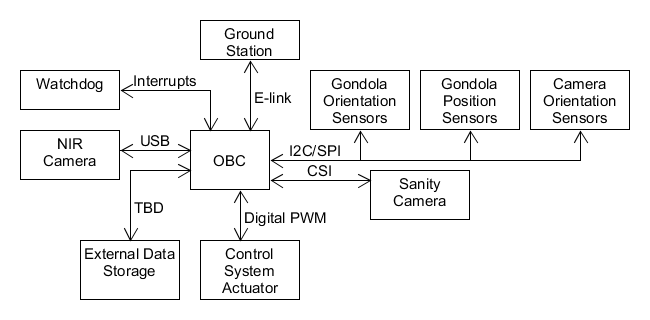
\includegraphics[width=.9\textwidth]{4-experiment-design/img/software/process-overview.png}
	\caption{Relations between On-Board Computer and connected components.}
	\label{fig:software-process-overview}
\end{figure}

All external components connected to the On-Board Computer and their interface are displayed in figure \ref{fig:software-process-overview}. The sanity camera provides an overview of the experiment and captures images on demand. The guiding camera provides an overall view in the direction the telescope is pointing and is also used as a star tracker to determine the gondola attitude. \st{A secondary microcontroller will be used to support the high sampling frequency needed for the gyroscopes. This microcontroller will be polled by the OBC.}

\paragraph{b)} General and safety related concepts

To ensure that the software is not erroneous rigorous testing will be done during development and after completion. A watchdog timer will be used to avoid software freezing. This timer will reset the On-Board Computer if it is not itself reset by the software within a certain period.

\paragraph{c)} Interfaces

If connection to ground is available, images compressed with a lossless compression will be sent down over the E-link over the course of the experiment. If the storage were to fail on touchdown for any reason, this would mean that not all data is lost. All communications over the E-link will be done using TCP to ensure that packet loss won't corrupt data.

\begin{table}[H]
	\centering
	\begin{tabular}{l|l}
		\textbf{Component}
		& \textbf{Interface} \\ \hline
		Ground Station
		& E-link             \\
		NIR Camera
		& USB                \\
		Guiding Camera
		& USB                \\
		Gondola GPS
		& SPI                \\
		Telescope Gyroscope
		& I2C                \\
		Telescope Encoders
		& I2C                \\
		Controller Actuators
		& I2C                \\
		Thermal Sensors
		& I2C				 \\
		Heaters \& Coolers
		& I2C
	\end{tabular}
	\caption{Table showing the interface that each external component was connected with. This is also visually represented in figure \ref{fig:software-process-overview}.}
	\label{tab:software-interfaces}
\end{table}


All housekeeping data will be stored in the form of text documents. This data will be transmitted to ground periodically. In the beginning of observations, images from the guiding camera will also be transmitted to verify that the system is working as intended. In the case that the images from the guiding camera are not as expected, an image from the sanity camera can be transmitted on demand. This is the only case a sanity image would be transmitted.

So long as there is additional headroom in the link budget, images from the NIR camera will be transmitted to ground. How many and when images are transmitted as well as an upper limit on the data rate if needed shall be controlled from ground. A minimum bandwidth of 300\,kbit/s is required for sensor data and guiding images. Once the initial guiding images has been received and verified, the nominal bandwidth required to transmit 10 images per hour is 500\,kbit/s. Any available bandwidth above that can be used to transmit additional images.

\newpage
The telecommands are very small compared to the telemetry. In the worst case scenario the command size is in the kbit range after all communication overhead is added. The following points shall be controllable from the ground station:

\begin{itemize}
	\item Rebooting the entire system.
	\item Updating the list of targets and their priorities.
	\item Calibrating the tracking to remove any offsets that may have appeared.
	\item Choosing how fast and how many NIR images will be transmitted.
	\item Setting camera settings such as exposure time and sensor gain.
	\item On-command image capturing with the guiding or sanity cameras.
\end{itemize}

\paragraph{d)} Data acquisition and storage

All data will be compressed using zstd, a lossless compression. The resulting compression ratio is heavily dependent on the contents of the data. A ratio of 2:1 (original data size to compressed) is used as a rough estimate from testing.

The main bulk of data handled is the images taken by the cameras. Housekeeping data such as positioning, camera direction, time, etc will also be stored along with the images. The On-Board Computer has one SD card used for the OS and temporary storage. For the external data storage two SD cards are used for redundancy purposes. All data shall be saved on these external SD-cards.

Both the NIR camera and the guiding camera have a colour depth of 12\,bits, but the image file format demands 16\,bits\,per\,pixel. This results in extra zero-padding on the data. However as this appears regularly, the compression algorithm can easily reduce the size overhead greatly.

As the NIR camera has a resolution of $5496 * 3672$ and 16\,bits\,per\,pixel, the raw image compressed size will be roughly 20\,MB. For a 4\,hour float phase and an exposure time of 30\,s a total of  9.69\,GB is required in on-board data storage for the images. An exposure time of 30\,s can't be guaranteed e.g. due to movements of the gondola. If the exposure time is dropped to 10\,s the total amount of data for continuous image capturing is 29\,GB.

The guiding camera has a resolution of $1936 * 1096$ and 16\,bits\,per\,pixel, leading to a raw image compressed size of roughly 2.1\,MB. If the guiding camera is sampled every 10\,s the total data required for the images is 3\,GB.

As the housekeeping data is negligible in size compared to the images and as the sanity images are only taken on demand, an SD-card size of 64\,GB will be sufficient for all data storage.

With a maximum of 1\,Mbit per second data transfer rate to ground it takes at least 161.5\,s to transfer one image compressed losslessly to 50\,\% of original size. This means that with little down time between observations and for most exposure times, not all images can be transmitted to ground.

The minimum data rate to the external storage required to save NIR images every 30\,s, guiding camera images every 10\,s, and sensor data polled each second is 900\,kbit/s.


\paragraph{e)} Process Flow

The system can either start in a testing mode, or in normal operation. The testing mode is used for pre-flight tests to ensure that all systems work as expected. Afterwards the system shall enter a sleep mode, a low activity state, with the camera in a safe launch position. During the ascent the thermal control system shall be running to ensure that all components of the experiment are within nominal temperature ranges.

When the float phase is reached, the system will wake. This is done by tracking the altitude of the gondola using GPS data. After wake-up the system shall find its orientation and the position of the sun. Finally tracking and observation can start.

Astronomical targets are prioritised. The software shall track and observe the highest priority target within the field of view with varying camera settings until one of the following events happen:

\begin{itemize}
	\item Current target leaves operational field of view.
	\item A higher priority target enters the field of view.
\end{itemize}

If one of the aforementioned events happens, the software will switch current target following prioritisation. While observing targets, the On-Board Software shall store images and housekeeping data. If connection to ground is available this data shall be compressed using a lossless compression method and sent to ground.

At the end of the floating phase the camera shall be oriented in a landing position and the system shall shut down. Figure \ref{fig:software-activity-diagram} shows the complete process flow. Figure \ref{fig:software-state-diagram} shows a simple state diagram for the experiment. Observations are done in the Normal state. In the rare case of a software freeze, it will be reset without entering sleep mode.

\begin{figure}[H]
    \centering
    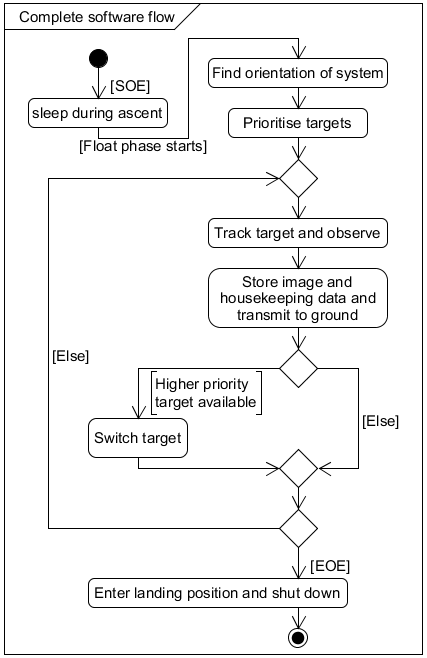
\includegraphics[width=.5\textwidth]{4-experiment-design/img/software/activity-diagram.png}
    \caption{Activity diagram describing the complete software flow. Here the internal actions SOE and EOE refer to when the software starts, i.e. on the launch pad, and shuts down respectively. This is done independently and therefore requires no activity from the gondola.}
    \label{fig:software-activity-diagram}
\end{figure}

\begin{figure}[H]
	\centering
	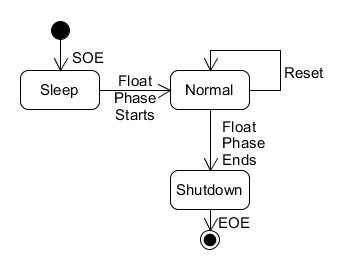
\includegraphics[width=.7\textwidth]{4-experiment-design/img/software/state-diagram.png}
	\caption{State diagram for On-Board Software.}
	\label{fig:software-state-diagram}
\end{figure}

\clearpage
\paragraph{f)} Modularisation and pseudo code

\begin{figure}[H]
	\centering
	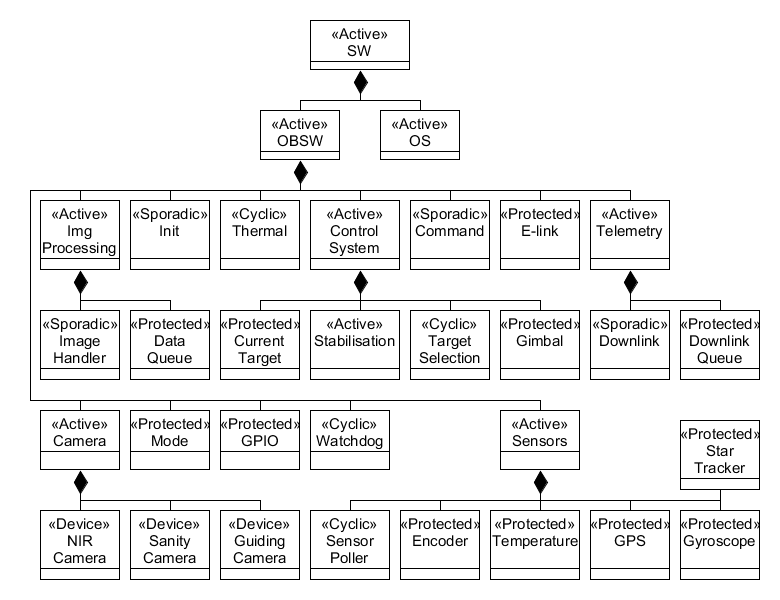
\includegraphics[width=\textwidth]{4-experiment-design/img/software/composition-tree.png}
	\caption{Composition tree of On-Board Software.}
	\label{fig:software-composition-tree}
\end{figure}

Figure \ref{fig:software-composition-tree} shows how the complete software is modularised. Each component is described below.

\begin{itemize}

	\item Camera: Parent
		\begin{itemize}
			\item Guiding Camera: Communication link to the guiding camera.
			\item NIR Camera: Communication link to the NIR camera.
			\item Sanity Camera: Communication link to the sanity camera.
		\end{itemize}

	\item Command: Module responsible for handling incoming commands from ground.

	\item E-link: Module responsible for communications over the E-link interface.

    \item GPIO: Module responsible for communications through the Raspberry Pi GPIO.

	\item Img Processing: Image processing, parent
		\begin{itemize}
			\item Data Queue: Buffer to hold camera data until Handler is ready
			\item Image Handler: Module processing and storing images taken by camera.
		\end{itemize}

	\item Init: Module initialising each component.

	\item Mode: Module responsible for the current state of the software.

	\item Sensors: Parent
		\begin{itemize}
            \item Encoder: Module holding encoder data.
            \item GPS: Module holding GPS data.
            \item Gyroscope: Module holding gyroscope data.
			 \item Sensor Poller: Module responsible for polling sensors.
            \item Star Tracker: Module holding absolute attitude obtained from the star tracker.
			\item Temperature: Thermal sensors.
		\end{itemize}

	\item Telemetry: Parent
		\begin{itemize}
			\item Downlink: Module responsible for sending telemetry to ground.
			\item Downlink Queue: Buffer to hold telemetry messages.
		\end{itemize}

	\item Thermal: Module responsible for active thermal control

	\item Control System: Parent
		\begin{itemize}
			\item Current Target: Module holding the current target to be observed.
			\item Controller: Module responsible for keeping camera on target.
			\item Gimbal: Module providing an interface to the gimbal motors.
			\item Target Selection: Module responsible for keeping track of target prioritisation and positioning as well as controlling the main camera.
		\end{itemize}

	\item Watchdog: Timer to reset watchdog.

\end{itemize}

\subsubsection{Implementation}

The code for the On-Board Software shall be implemented in C. An operating system will be used to enable the modularisation required. The chosen operating system is Linux with the Preempt RT kernel patch. Additional libraries, such as the ASI SDK library used for controlling the cameras, will be needed. The compression used for the telemetry is supplied by the zstd library.



\subsubsection{Control system}
The main task of the control system is selecting and tracking the astronomical targets and stabilising the telescope during exposure. Other tasks include minor tasks like the thermal control of the CMOS sensor and the electronics box as well as control of the actuators. A general overview of the control loop for tracking \& stabilisation is given in figure  \mbox{\ref{fig::software::control_loop}} below. The thermal control loop is sketched in chapter \mbox{\ref{Thermal_section}}.

\paragraph{Selecting and tracking targets}

The selection and tracking of targets is done by using the current time, position (GPS) and orientation star tracker and gyroscope) of the gondola. Once a suitable target in the operational field of view is selected, it is tracked during exposure. This includes the compensation of the following motions:
\begin{itemize}
	\item Time-dependent rotational motion of the astronomical targets in the sky. This will be continuously compensated during exposure using models and/or interpolation of tables.
	\item Position-dependent rotational motion of the astronomical targets in the sky. This will be corrected once for every picture, using the GPS data.
	\item Rotation of the gondola in the z-axis; can be corrected during exposure using a gyroscope sensor.
\end{itemize}

Due to the nature of the motion of astronomical targets, it is necessary to use a 3-axis gimbal.

The three axes and the names for the rotation axes are shown in figure \mbox{\ref{fig::software::Yaw_Pitch_Roll}}.

\textbf{Selection of targets}

The selection of targets is based on the operational field of view (the area of the sky where the telescope is able to look at) and prioritisation parameters of the possible targets within this field of view. The operational field of view is determined by using the sensor data from the orientation sensor (star tracker). Using a star tracker will provide an accurate absolute attitude determination system to ensure that the celestial object of interest is actually in the field of view of the telescope when it is pointed there. Compared to the gyroscopes that have a much higher angular resolution, the attitude determination system does not show any drift over time and does therefore not need to be calibrated during flight.

Prioritisation parameters include the brightness of the object (brighter objects are expected to yield better results due to higher SNR), the location of the object within the operational field of view (objects near the centre of the field of view are favoured because they are less likely to rotate out of the field of view during exposure) and the number of exposures already taken (objects should be imaged more than once in order to be able to compare and verify the obtained data, but not more often than ten times during the flight). 

As the location of the astronomical targets changes with time and position of the gondola, these two parameters also need to be taken into account (for determination see paragraph Astronomical targets). Once a target is selected, this part of the control system will be deactivated until the picture was taken or the control loop is re-initialised.

The 4 chosen prioritisation parameters are:
\begin{itemize}
	\item No. of exposures already taken (exposure parameter)
	\item Magnitude of the target (constant)
	\item Position parameter
	\item Type of target  (defined scientific parameter, constant)
\end{itemize}

The exposure parameter depends on the number of images of the target that have already been taken, and is defined as follows: \texttt{exp\_ param\_ list = [1,2,3,4,4,4,3,2,1,1,1]} for 0 to 9 exposures respectively, and 0 for all other. This ensures that not more than 10 images are taken (maximum defined in the scientific requirements) and that targets with more than 2 exposures are prioritised in order to get sufficient scientific data of one target.

The magnitude of the target is defined by the target itself and is therefore constant. Typical values range from 3 to 10 for the chosen targets. The higher the value the brighter the target, and therefore more suitable to observe.

The position parameter depends on the gondola attitude and is recalculated based on the current time, position and attitude each time. It is then calculated as follows: if the absolute difference between the gondola attitude and the target position is smaller than a set value (e.\,g.~maximum telescope range - $\ang{30}$) it is defined as 

\begin{align*}
	\left|\text{gondola attitude} - \text{target position} \right|
\end{align*}
otherwise as zero. This means that no targets that are outside the field of view are chosen, and the most central targets are preferred in order to minimise the risk of the target rotating out of the field of view during exposure.

The type of target (nebula/galaxy/open cluster/globular cluster) prioritises nebulae and galaxies to cluster. The prioritisation order is \texttt{type\_ param\_ list = [4,3,2,1]} for the order mentioned above.

To get a final prioritisation value for each target, all prioritisation parameters are multiplied. This ensures that targets outside the field of view as well as targets with 10 exposures are not taken into consideration any more, as the result is 0. The target with the highest calculated prioritisation value is selected for the next exposure.



\textbf{Tracking of astronomical targets}

The time-dependent and the position-dependent rotational motion of the astronomical targets are calculated by using an astronomical model and provides the control input for the subsequent stages of the control system. Because the state vectors for this model are time (internal clock) and position (GPS) and the input vector is the selected target (defined in the system, not a variable state for the exposure of one image), the state vectors cannot be affected by the control system (not controllable). Therefore, no dedicated feedback loop is used for this part of the control system. However, the input data from the GPS may be filtered before use. The output vector then provides the input for the compensation of rotation (of the gondola in the z-axis) and the stabilisation of the gimbal.

The astronomical model used to determine the current position of the targets is the Alt Az (Altitude Azimuth) reference frame. It defines the position of the astronomical target with respect to geographic north and zenith and depends on current the time, date and position of the observer. It is calculated based on the RA DEC (Right Ascension, Declination) of the astronomical target. The formulas required for this conversion are given in \mbox{\cite{RaDec2AltAz}}.

\textbf{Rotation of the gondola}

The uncontrolled rotational motion of the gondola around the z-axis can be directly compensated by actuating the corresponding gimbal axis (yaw). This will be achieved by a PID control. As the same axis will also be actuated during the stabilisation process, it will be merged with the control loop for the stabilisation. As the required accuracy for detecting the rotation of the gondola is very high, the gyroscopes are used to provide the input (see stabilisation for more detail).


\paragraph{Stabilisation of the gimbal}
The stabilisation of the gimbal only needs to be active during exposure in order to avoid blurred pictures. It is responsible for compensating all kinds of small-scale, unpredicted movements of the gondola. In order to achieve this, an active feedback loop that requires information about the gondola movements is needed. This information is gathered by using accelerometers and gyroscopes for all 3 axes.

After the target is selected, the gyroscopes are reset so there is no offset-error and the best accuracy can be achieved. With this setup, it is possible to measure the movements of the gondola with an accuracy higher than the corresponding angular resolution of one pixel. Once the gyroscopes are reset the value of the attitude determination system is held constant within the control system, because the accuracy of the gyroscopes is orders of magnitude higher than that of the attitude determination system. 

In addition to the gyroscopes, the encoders are used to obtain the actual position of the telescope within the gondola and therefore provide a second set of data for the feedback loop. The sensor data is filtered by a Kalman filter to decrease the sensor noise and deduce the current orientation of the telescope as well as the motion of the gondola with a high precision.

The control of the gimbal (tracking and stabilisation as well as compensation of the gondola rotation for the yaw axis) is done by a separate PID control for each axis. The output of the controller is the required speed for the actuating motor of the respective axis. This information is then processed by the motor controller that calculates the required input currents for the motors.

The stabilisation algorithm is written in C as the most of the OBSW. The team refrained from using third party libraries, so the whole stabilisation code is built using standard C libraries. The analisys will be conducted on a Simulink model and acquired PID values are tested on an instrument during integration tests.

%\begin{figure}%[h]
%	\centering
%	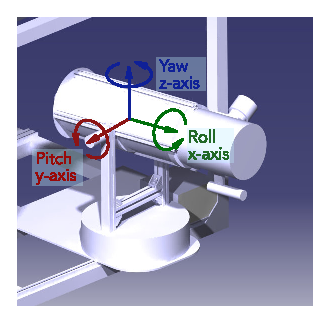
\includegraphics[width = 0.4\textwidth]{4-experiment-design/img/software/Yaw_Pitch_Roll.eps}
%	\caption{\hl{Yaw, Pitch and Roll angles of the gimbal [New figure]}}
%	\label{fig::software::Yaw_Pitch_Roll}
%\end{figure}

\newpage
\begin{landscape}
	\begin{figure}
		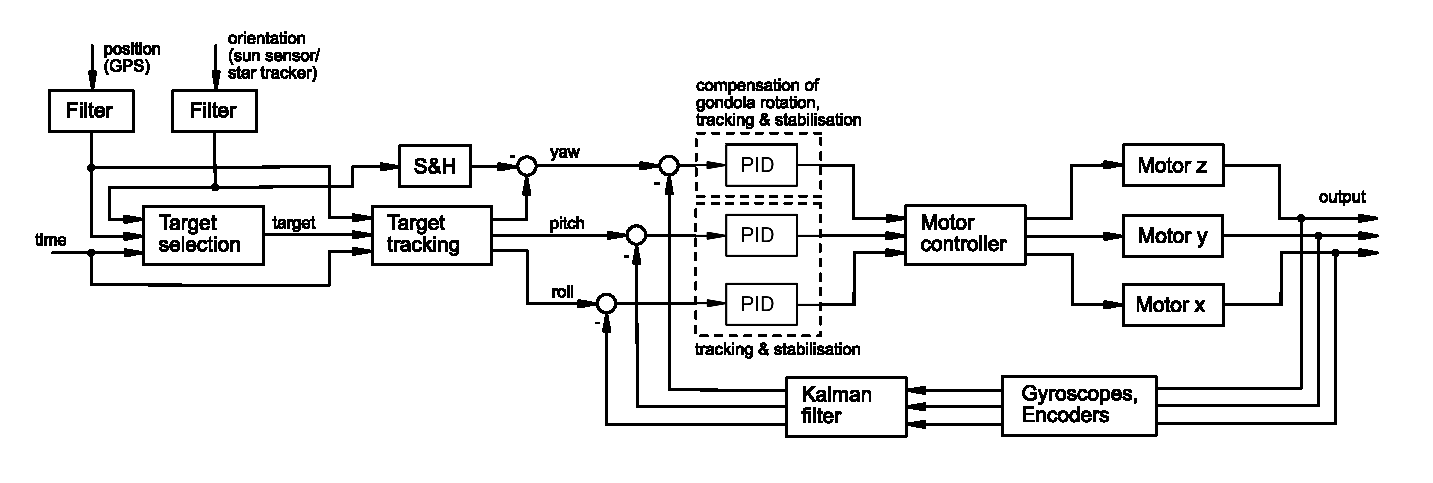
\includegraphics[width=\linewidth]{4-experiment-design/img/software/Control_loop.eps}
		\caption{Control loop of the experiment}
		\label{fig::software::control_loop}
	\end{figure}
\end{landscape}


\raggedbottom
